\documentclass[]{article}
\usepackage{lmodern}
\usepackage{amssymb,amsmath}
\usepackage{ifxetex,ifluatex}
\usepackage{fixltx2e} % provides \textsubscript
\ifnum 0\ifxetex 1\fi\ifluatex 1\fi=0 % if pdftex
  \usepackage[T1]{fontenc}
  \usepackage[utf8]{inputenc}
\else % if luatex or xelatex
  \ifxetex
    \usepackage{mathspec}
  \else
    \usepackage{fontspec}
  \fi
  \defaultfontfeatures{Ligatures=TeX,Scale=MatchLowercase}
\fi
% use upquote if available, for straight quotes in verbatim environments
\IfFileExists{upquote.sty}{\usepackage{upquote}}{}
% use microtype if available
\IfFileExists{microtype.sty}{%
\usepackage{microtype}
\UseMicrotypeSet[protrusion]{basicmath} % disable protrusion for tt fonts
}{}
\usepackage[margin=1in]{geometry}
\usepackage{hyperref}
\hypersetup{unicode=true,
            pdftitle={introduccion a markdown},
            pdfauthor={christian arcos},
            pdfborder={0 0 0},
            breaklinks=true}
\urlstyle{same}  % don't use monospace font for urls
\usepackage{color}
\usepackage{fancyvrb}
\newcommand{\VerbBar}{|}
\newcommand{\VERB}{\Verb[commandchars=\\\{\}]}
\DefineVerbatimEnvironment{Highlighting}{Verbatim}{commandchars=\\\{\}}
% Add ',fontsize=\small' for more characters per line
\usepackage{framed}
\definecolor{shadecolor}{RGB}{248,248,248}
\newenvironment{Shaded}{\begin{snugshade}}{\end{snugshade}}
\newcommand{\KeywordTok}[1]{\textcolor[rgb]{0.13,0.29,0.53}{\textbf{#1}}}
\newcommand{\DataTypeTok}[1]{\textcolor[rgb]{0.13,0.29,0.53}{#1}}
\newcommand{\DecValTok}[1]{\textcolor[rgb]{0.00,0.00,0.81}{#1}}
\newcommand{\BaseNTok}[1]{\textcolor[rgb]{0.00,0.00,0.81}{#1}}
\newcommand{\FloatTok}[1]{\textcolor[rgb]{0.00,0.00,0.81}{#1}}
\newcommand{\ConstantTok}[1]{\textcolor[rgb]{0.00,0.00,0.00}{#1}}
\newcommand{\CharTok}[1]{\textcolor[rgb]{0.31,0.60,0.02}{#1}}
\newcommand{\SpecialCharTok}[1]{\textcolor[rgb]{0.00,0.00,0.00}{#1}}
\newcommand{\StringTok}[1]{\textcolor[rgb]{0.31,0.60,0.02}{#1}}
\newcommand{\VerbatimStringTok}[1]{\textcolor[rgb]{0.31,0.60,0.02}{#1}}
\newcommand{\SpecialStringTok}[1]{\textcolor[rgb]{0.31,0.60,0.02}{#1}}
\newcommand{\ImportTok}[1]{#1}
\newcommand{\CommentTok}[1]{\textcolor[rgb]{0.56,0.35,0.01}{\textit{#1}}}
\newcommand{\DocumentationTok}[1]{\textcolor[rgb]{0.56,0.35,0.01}{\textbf{\textit{#1}}}}
\newcommand{\AnnotationTok}[1]{\textcolor[rgb]{0.56,0.35,0.01}{\textbf{\textit{#1}}}}
\newcommand{\CommentVarTok}[1]{\textcolor[rgb]{0.56,0.35,0.01}{\textbf{\textit{#1}}}}
\newcommand{\OtherTok}[1]{\textcolor[rgb]{0.56,0.35,0.01}{#1}}
\newcommand{\FunctionTok}[1]{\textcolor[rgb]{0.00,0.00,0.00}{#1}}
\newcommand{\VariableTok}[1]{\textcolor[rgb]{0.00,0.00,0.00}{#1}}
\newcommand{\ControlFlowTok}[1]{\textcolor[rgb]{0.13,0.29,0.53}{\textbf{#1}}}
\newcommand{\OperatorTok}[1]{\textcolor[rgb]{0.81,0.36,0.00}{\textbf{#1}}}
\newcommand{\BuiltInTok}[1]{#1}
\newcommand{\ExtensionTok}[1]{#1}
\newcommand{\PreprocessorTok}[1]{\textcolor[rgb]{0.56,0.35,0.01}{\textit{#1}}}
\newcommand{\AttributeTok}[1]{\textcolor[rgb]{0.77,0.63,0.00}{#1}}
\newcommand{\RegionMarkerTok}[1]{#1}
\newcommand{\InformationTok}[1]{\textcolor[rgb]{0.56,0.35,0.01}{\textbf{\textit{#1}}}}
\newcommand{\WarningTok}[1]{\textcolor[rgb]{0.56,0.35,0.01}{\textbf{\textit{#1}}}}
\newcommand{\AlertTok}[1]{\textcolor[rgb]{0.94,0.16,0.16}{#1}}
\newcommand{\ErrorTok}[1]{\textcolor[rgb]{0.64,0.00,0.00}{\textbf{#1}}}
\newcommand{\NormalTok}[1]{#1}
\usepackage{graphicx,grffile}
\makeatletter
\def\maxwidth{\ifdim\Gin@nat@width>\linewidth\linewidth\else\Gin@nat@width\fi}
\def\maxheight{\ifdim\Gin@nat@height>\textheight\textheight\else\Gin@nat@height\fi}
\makeatother
% Scale images if necessary, so that they will not overflow the page
% margins by default, and it is still possible to overwrite the defaults
% using explicit options in \includegraphics[width, height, ...]{}
\setkeys{Gin}{width=\maxwidth,height=\maxheight,keepaspectratio}
\IfFileExists{parskip.sty}{%
\usepackage{parskip}
}{% else
\setlength{\parindent}{0pt}
\setlength{\parskip}{6pt plus 2pt minus 1pt}
}
\setlength{\emergencystretch}{3em}  % prevent overfull lines
\providecommand{\tightlist}{%
  \setlength{\itemsep}{0pt}\setlength{\parskip}{0pt}}
\setcounter{secnumdepth}{0}
% Redefines (sub)paragraphs to behave more like sections
\ifx\paragraph\undefined\else
\let\oldparagraph\paragraph
\renewcommand{\paragraph}[1]{\oldparagraph{#1}\mbox{}}
\fi
\ifx\subparagraph\undefined\else
\let\oldsubparagraph\subparagraph
\renewcommand{\subparagraph}[1]{\oldsubparagraph{#1}\mbox{}}
\fi

%%% Use protect on footnotes to avoid problems with footnotes in titles
\let\rmarkdownfootnote\footnote%
\def\footnote{\protect\rmarkdownfootnote}

%%% Change title format to be more compact
\usepackage{titling}

% Create subtitle command for use in maketitle
\providecommand{\subtitle}[1]{
  \posttitle{
    \begin{center}\large#1\end{center}
    }
}

\setlength{\droptitle}{-2em}

  \title{introduccion a markdown}
    \pretitle{\vspace{\droptitle}\centering\huge}
  \posttitle{\par}
    \author{christian arcos}
    \preauthor{\centering\large\emph}
  \postauthor{\par}
      \predate{\centering\large\emph}
  \postdate{\par}
    \date{April 24, 2019}

\usepackage{booktabs}
\usepackage{longtable}
\usepackage{array}
\usepackage{multirow}
\usepackage{wrapfig}
\usepackage{float}
\usepackage{colortbl}
\usepackage{pdflscape}
\usepackage{tabu}
\usepackage{threeparttable}
\usepackage{threeparttablex}
\usepackage[normalem]{ulem}
\usepackage{makecell}
\usepackage{xcolor}

\begin{document}
\maketitle

\begin{center}\rule{0.5\linewidth}{\linethickness}\end{center}

\begin{Shaded}
\begin{Highlighting}[]
\KeywordTok{library}\NormalTok{(htmlTable)}
\KeywordTok{library}\NormalTok{(knitr)}
\KeywordTok{library}\NormalTok{(kableExtra)}
\end{Highlighting}
\end{Shaded}

\subsection{R Markdown}\label{r-markdown}

This is an R Markdown document. Markdown is a simple formatting syntax
for authoring HTML, PDF, and MS Word documents. For more details on
using R Markdown see \url{http://rmarkdown.rstudio.com}.

When you click the \textbf{Knit} button a document will be generated
that includes both content as well as the output of any embedded R code
chunks within the document. You can embed an R code chunk like this:

\begin{Shaded}
\begin{Highlighting}[]
\KeywordTok{summary}\NormalTok{(cars)}
\end{Highlighting}
\end{Shaded}

\begin{verbatim}
##      speed           dist       
##  Min.   : 4.0   Min.   :  2.00  
##  1st Qu.:12.0   1st Qu.: 26.00  
##  Median :15.0   Median : 36.00  
##  Mean   :15.4   Mean   : 42.98  
##  3rd Qu.:19.0   3rd Qu.: 56.00  
##  Max.   :25.0   Max.   :120.00
\end{verbatim}

\section{HTML Contents}\label{html-contents}

\url{http://christianArcos.com}

esto es un nuevo parrafo escrito con etiquetas de HTML

Ventajas

Inconcenientes

es facil de utilizar

necesita precision y planning

puede exportara multiples formatos

necesitamos conocer otras tecnologias

\section{incrustar codigo}\label{incrustar-codigo}

Se puede definir cualquier codigo en \emph{R} haciedno uso de los tres
acentos agudos. El paramtero echo=FALSE, indica que el chunk no se
mostrara en el documento.

\begin{itemize}
\tightlist
\item
  Tambien se pueden definir las opciones de mostrar o no los chunks de
  forma global en todo el documento.
\item
  Tambien se puede definir una cache global para no sobrecargar la
  generacion de ficheros
\item
  se puede definir el directorio rais de donde cargar cualquier fichero
  de datos haciendo uso de l parametro root.dir

  \begin{itemize}
  \tightlist
  \item
    hola
  \end{itemize}
\end{itemize}

\subsection{Loading Data}\label{loading-data}

\begin{Shaded}
\begin{Highlighting}[]
\NormalTok{auto <-}\StringTok{ }\KeywordTok{read.csv}\NormalTok{(}\StringTok{"../../data/tema10/auto-mpg.csv"}\NormalTok{)}
\end{Highlighting}
\end{Shaded}

Despues de cargar los datos solemos mirar informacion acerca de los
primeros elementos del data frame, la estructura de las columnas del
mismo e incluso un resumen de los estadisticos basicos de cada una

\begin{Shaded}
\begin{Highlighting}[]
\KeywordTok{htmlTable}\NormalTok{(}\KeywordTok{head}\NormalTok{(auto))}
\end{Highlighting}
\end{Shaded}

No

mpg

cylinders

displacement

horsepower

weight

acceleration

model\_year

car\_name

1

1

28

4

140

90

2264

15.5

71

chevrolet vega 2300

2

2

19

3

70

97

2330

13.5

72

mazda rx2 coupe

3

3

36

4

107

75

2205

14.5

82

honda accord

4

4

28

4

97

92

2288

17

72

datsun 510 (sw)

5

5

21

6

199

90

2648

15

70

amc gremlin

6

6

23

4

115

95

2694

15

75

audi 100ls

\begin{Shaded}
\begin{Highlighting}[]
\KeywordTok{str}\NormalTok{(auto)}
\end{Highlighting}
\end{Shaded}

\begin{verbatim}
## 'data.frame':    398 obs. of  9 variables:
##  $ No          : int  1 2 3 4 5 6 7 8 9 10 ...
##  $ mpg         : num  28 19 36 28 21 23 15.5 32.9 16 13 ...
##  $ cylinders   : int  4 3 4 4 6 4 8 4 6 8 ...
##  $ displacement: num  140 70 107 97 199 115 304 119 250 318 ...
##  $ horsepower  : int  90 97 75 92 90 95 120 100 105 150 ...
##  $ weight      : int  2264 2330 2205 2288 2648 2694 3962 2615 3897 3755 ...
##  $ acceleration: num  15.5 13.5 14.5 17 15 15 13.9 14.8 18.5 14 ...
##  $ model_year  : int  71 72 82 72 70 75 76 81 75 76 ...
##  $ car_name    : Factor w/ 305 levels "amc ambassador brougham",..: 66 184 165 86 8 18 11 79 42 112 ...
\end{verbatim}

\begin{Shaded}
\begin{Highlighting}[]
\KeywordTok{summary}\NormalTok{(auto)}
\end{Highlighting}
\end{Shaded}

\begin{verbatim}
##        No             mpg          cylinders      displacement  
##  Min.   :  1.0   Min.   : 9.00   Min.   :3.000   Min.   : 68.0  
##  1st Qu.:100.2   1st Qu.:17.50   1st Qu.:4.000   1st Qu.:104.2  
##  Median :199.5   Median :23.00   Median :4.000   Median :148.5  
##  Mean   :199.5   Mean   :23.51   Mean   :5.455   Mean   :193.4  
##  3rd Qu.:298.8   3rd Qu.:29.00   3rd Qu.:8.000   3rd Qu.:262.0  
##  Max.   :398.0   Max.   :46.60   Max.   :8.000   Max.   :455.0  
##                                                                 
##    horsepower        weight      acceleration     model_year   
##  Min.   : 46.0   Min.   :1613   Min.   : 8.00   Min.   :70.00  
##  1st Qu.: 76.0   1st Qu.:2224   1st Qu.:13.82   1st Qu.:73.00  
##  Median : 92.0   Median :2804   Median :15.50   Median :76.00  
##  Mean   :104.1   Mean   :2970   Mean   :15.57   Mean   :76.01  
##  3rd Qu.:125.0   3rd Qu.:3608   3rd Qu.:17.18   3rd Qu.:79.00  
##  Max.   :230.0   Max.   :5140   Max.   :24.80   Max.   :82.00  
##                                                                
##            car_name  
##  ford pinto    :  6  
##  amc matador   :  5  
##  ford maverick :  5  
##  toyota corolla:  5  
##  amc gremlin   :  4  
##  amc hornet    :  4  
##  (Other)       :369
\end{verbatim}

\subsubsection{Plot data}\label{plot-data}

You can also embed plots, for example:

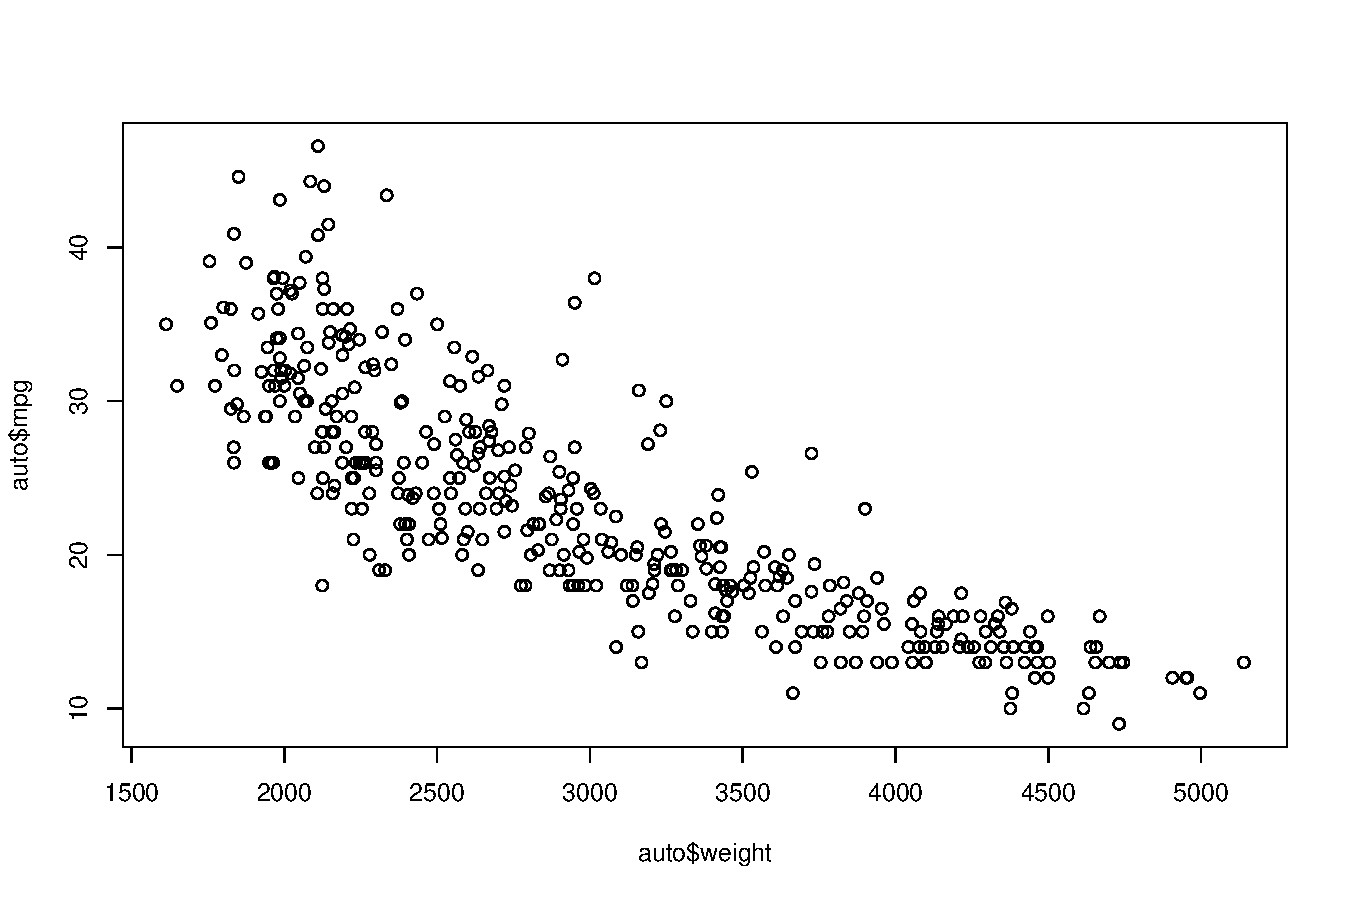
\includegraphics{intro_markdown_files/figure-latex/disperssion-1.pdf}

Note that the \texttt{echo\ =\ FALSE} parameter was added to the code
chunk to prevent printing of the R code that generated the plot.

\subsubsection{Inline R}\label{inline-r}

hemos hecho uso de un data frame que contiene 398 muestras de coches y
cada uno de ellos tiene 9 variables.


\end{document}
